\documentclass[11pt,a4paper]{article}

\usepackage[T1]{fontenc}
\usepackage[utf8]{inputenc}
\usepackage{lmodern}
\usepackage{microtype}
\usepackage{amsmath,amssymb,amsthm,mathtools,bm}
\usepackage{booktabs,array,tabularx,longtable}
\usepackage{graphicx,float,caption}
\usepackage{xcolor}
\usepackage[margin=23mm]{geometry}
\usepackage{enumitem}
\usepackage{fancyhdr}
\usepackage{hyperref}

\definecolor{finblue}{HTML}{1F5A99}
\definecolor{finorange}{HTML}{C45A00}
\definecolor{fingreen}{HTML}{19733A}
\definecolor{finred}{HTML}{A61B1B}
\definecolor{finpurple}{HTML}{6B3FA0}
\definecolor{finsoft}{HTML}{F2F5F8}
\definecolor{fingray}{HTML}{4E5964}

\hypersetup{
  colorlinks=true,
  linkcolor=finblue,
  citecolor=fingreen,
  urlcolor=finblue,
  pdftitle={FIN Programs P488-P496: Low-Compute Analytical Research},
  pdfauthor={Krzysztof Żuchowski},
  pdfsubject={Persistent spectral cycles, relational time, adaptive Stieltjes memory, dynamic kernel carriers, and topology boundaries},
  pdfkeywords={FIN, nadsoliton, spectral clock, Stieltjes function, Schur complement, fractal fixed point, resonance, topological defect, operational identifiability}
}

\pagestyle{fancy}
\fancyhf{}
\fancyhead[L]{\small FIN Programs P488--P496}
\fancyhead[R]{\small Release 10.49}
\fancyfoot[C]{\thepage}
\setlength{\headheight}{14pt}

\newtheorem{theorem}{Theorem}[section]
\newtheorem{proposition}[theorem]{Proposition}
\newtheorem{corollary}[theorem]{Corollary}
\theoremstyle{definition}
\newtheorem{definition}[theorem]{Definition}
\theoremstyle{remark}
\newtheorem{remark}[theorem]{Remark}

\newcommand{\C}{\mathbb C}
\newcommand{\R}{\mathbb R}
\newcommand{\one}{\bm 1}
\newcommand{\Tr}{\operatorname{Tr}}
\newcommand{\status}[2]{\textcolor{#1}{\textbf{[#2]}}}
\newcommand{\proven}{\status{fingreen}{PROVEN}}
\newcommand{\strong}{\status{finblue}{STRONG EVIDENCE}}
\newcommand{\moderate}{\status{finorange}{MODERATE EVIDENCE}}
\newcommand{\speculative}{\status{finpurple}{SPECULATIVE}}
\newcommand{\refuted}{\status{finred}{REFUTED}}
\newcommand{\conditional}{\status{fingray}{CONDITIONAL}}
\newcommand{\claimbox}[1]{\begin{center}\fcolorbox{finblue}{finsoft}{\parbox{0.91\textwidth}{#1}}\end{center}}

\setlist[itemize]{leftmargin=*,topsep=3pt,itemsep=2pt}
\setlist[enumerate]{leftmargin=*,topsep=3pt,itemsep=2pt}
\setlength{\emergencystretch}{2em}

\begin{document}
\hypersetup{pageanchor=false}

\begin{titlepage}
\centering
\vspace*{16mm}
{\Huge\bfseries FIN Programs P488--P496\par}
\vspace{5mm}
{\Large Low-Compute Analytical Research\par}
\vspace{3mm}
{\large Persistent spectral cycles, relational time, adaptive memory,\par}
{\large dynamic kernel carriers, topology, and operational identifiability\par}
\vspace{15mm}
{\Large Krzysztof Żuchowski\par}
\vspace{2mm}
{\normalsize Independent Researcher --- Fractal Information Theory Project\par}
{\normalsize ORCID: 0009-0002-0909-3613\par}
\vspace{10mm}
{\large FIN Release 10.49 --- Version 1.0.0\par}
{\large 10 August 2026\par}
\vfill
\begin{minipage}{0.90\textwidth}
\small
\textbf{Scope.} This report executes the nine recommendations from the FIN Theory Compendium that do not require a large Gröbner-basis elimination, a global exact cone optimization, laboratory access, or an external audit. P485, P487, and the global exact phase-face problem are deliberately excluded.

\medskip
\textbf{Evidence boundary.} Exact algebra, analytic derivations, small dense linear algebra, and synthetic finite records are admitted. No repository-generated record is represented as external physical evidence. New dynamical laws are labelled as supplied models rather than consequences of the frozen kernel.

\medskip
\textbf{Runtime.} The full numerical batch completed locally in approximately 32 seconds. Ten regression tests completed in 0.18 seconds.

\medskip
\textbf{Repository.} \url{https://github.com/hyconiek/Fractal-Nadsoliton-Theory}

\textbf{License.} CC BY 4.0.
\end{minipage}
\vfill
\end{titlepage}
\hypersetup{pageanchor=true}

\begin{abstract}
Nine low-compute FIN studies are executed. First, a new saturating strict spectral flow
\[
\dot\psi=(r-g|\psi|^2)\psi-iA\psi
\]
is constructed. Every constant-modulus Fourier eigenmode of the strict $\mathbb Z_{12}$ generator is an exact persistent rotating state. Five excited modes have strictly negative transverse exponents in the numerical linearization, while mode three has an additional neutral exponent. All have inverse participation ratio $1/12$, so the construction gives persistent coherent cycles but not a localized soliton.

The first excited cycle defines a local relational clock with dimensionless period $8.3317982424$. Its phase is invariant under simultaneous rescaling of generator and time, proving that the clock cannot select an absolute second. A positive log-parameter flow on the three-pole Stieltjes trace response preserves complete monotonicity and recovers the declared response to $1.31\times10^{-15}$ relative error, but its Jacobian condition number is $3.52\times10^7$ and the target/loss remain supplied.

An exact dynamic fractal fixed point is excluded for the declared normalized $C_{12},C_{24},C_{48},C_{96}$ attenuation-envelope contexts: the distinct visible pole counts are $3,6,12,24$, and the finite-size response discrepancies are nonzero and nonmonotone. The identity $A=sI-W$ proves that maximum coupling resonance is exactly minimum Dirichlet cost, whereas maximum temporal frequency reverses this ordering.

An exponent-lift completion automaton is proved to generate both Legacy* and strict formulas exactly for all integer distances and across three carrier sizes. It represents, but does not derive, the parameter transition; the naive linear parameter homotopy becomes a nonnegative-weight passive $C_{12}$ Laplacian only at sampled $t\ge0.93$. A topology audit proves that the scalar space $\C^{12}$ has no protected winding sectors; a nonvanishing phase field and refinement rule are additional obligations. Finally, coherence-sensitive Fourier measurements raise synthetic four-model classification from $0.5775/0.745$ to $1.0$ in the declared test, while a dependency-minimal exact checker replays the Dirichlet, Schur, resonance, and Legacy* recurrence identities.

The batch therefore constructs three useful missing mathematical objects---a persistent spectral cycle, a relational clock, and a class-preserving adaptive memory flow---but does not generate a localized nadsoliton, physical time, a learning objective, particle topology, or laboratory evidence.
\end{abstract}

\noindent\textbf{Status vocabulary.}
\proven{} denotes an analytic statement or exact finite replay under declared assumptions;
\strong{} denotes robust numerical or synthetic evidence;
\conditional{} denotes a theorem after a supplied dynamical or operational law;
\speculative{} denotes an open research interpretation;
\refuted{} denotes a scoped counterexample or no-go.

\tableofcontents
\newpage

\section{Executive results}

\claimbox{\textbf{Principal advance.} A minimal gain--saturation law turns every strict Fourier eigenmode into an exact persistent rotating state. This is the first result in the selected batch that mathematically realizes the ``information persists through self-reinforcement'' intuition. It is conditional on the new nonlinear law and does not yet realize spatial localization.}

\begin{longtable}{@{}p{0.07\textwidth}p{0.23\textwidth}p{0.39\textwidth}p{0.23\textwidth}@{}}
\caption{Programs, new objects, and terminal verdicts.}\\
\toprule
ID & New typed object & Main result & Status\\
\midrule
\endfirsthead
\toprule
ID & New typed object & Main result & Status\\
\midrule
\endhead
P488 & O192 Saturating Strict Spectral Limit-Cycle Flow & Exact persistent rotating modes; five excited modes strictly transversely damped numerically, one neutral; all delocalized. & \conditional{} / \strong\\
P489 & O193 Relational Spectral Phase Clock & Relative phase time exists modulo (8.3318); absolute scale remains a free orbit. & \proven\\
P490 & O194 Positive Stieltjes Parameter Learning Flow & Positivity and complete monotonicity are preserved; declared response recovered, but ill-conditioned. & \proven{} / \strong\\
P491 & O195 Normalized Dynamic Context Fingerprint & Exact fixed point excluded on the declared four-size family; no monotone convergence evidence. & \proven\\
P492 & O196 Resonance--Dirichlet Complementarity & Maximum $W$-coupling equals minimum $A$-cost; maximum $A$-frequency is different. & \proven\\
P493 & O197 Exponent-Lift Kernel Completion Automaton & Legacy* and strict are exact parameter points of one state map; no parameter source is created. & \proven\\
P494 & O198 Phase-Field Topology Obligation & Scalar kernel states do not possess protected winding sectors. & \proven\\
P495 & O199 Local Operational Identifiability Atlas & Coherence-sensitive records separate four declared synthetic dynamics; population records do not. & \strong\\
P496 & O200 Dependency-Minimal Algebraic Replay & Four core identities replayed exactly with standard-library rational arithmetic. & \proven{} in replay scope\\
\bottomrule
\end{longtable}

\section{Shared strict finite core}

On $V=\mathbb Z/12\mathbb Z$, let $W_{xx}=0$ and
\[
W_{xy}=\frac{\cos(0.18575d(x,y)+0.16250)}{1+d(x,y)^{1.8}},
\qquad A=sI-W,
\]
with cyclic distance and
\[
s=1.6603072787660986\ldots.
\]
All six sampled off-diagonal weights are positive, so
\[
\langle f,Af\rangle=\frac12\sum_{x,y}W_{xy}|f_x-f_y|^2\ge0.
\]
The gap and maximum eigenvalue are
\[
\lambda_1=0.7541211542070796,
\qquad
\lambda_{\max}=2.3421820411463004.
\]

This matrix is the fixed input to P488, P489, P490, P492, P494 and P495. P491 declares a separate positive attenuation-envelope refinement family; P493 keeps legacy and strict parameters separated inside one newly supplied state map.

\section{P488 --- a conditional persistent nadsoliton mechanism}

\subsection{The new nonlinear object}

The frozen strict matrix supports oscillation but does not supply gain, saturation or learning. Introduce the finite complex flow
\[
\boxed{\dot\psi_x=(r-g|\psi_x|^2)\psi_x-i(A\psi)_x},
\qquad r,g>0.
\]
The real term is uniform gain with local cubic saturation; the skew term is the strict unitary generator. The law is a newly supplied candidate, not a strict consequence.

\begin{theorem}[Exact strict spectral cycles]
Let $v_m(x)=12^{-1/2}e^{2\pi imx/12}$ and $Av_m=\lambda_mv_m$. Then
\[
\psi_m(t)=\sqrt{\frac{12r}{g}}\,e^{-i\lambda_mt}v_m
\]
is an exact solution. Every site has amplitude $\sqrt{r/g}$.
\end{theorem}

\begin{proof}
Every Fourier coordinate has equal modulus, so
\[
g|\psi_m(x)|^2=g\frac{12r/g}{12}=r.
\]
Gain and saturation cancel pointwise, leaving
\(
\dot\psi_m=-iA\psi_m=-i\lambda_m\psi_m
\).
\end{proof}

With $r=0.2$, $g=1$, exact equation residuals are below $3.0\times10^{-15}$. The inverse participation ratio is
\[
\sum_x|v_m(x)|^4=\frac1{12}
\]
for every mode. Thus the solutions persist but are maximally delocalized on the carrier.

\subsection{Linearized stability audit}

The real $24\times24$ co-rotating Jacobian was diagonalized for modes $0$ through $6$. One zero exponent is required by global phase symmetry. After removing it, the largest real parts are:

\begin{center}
\begin{tabular}{@{}rrrr@{}}
\toprule
Mode & Frequency & Period & Largest transverse real part\\
\midrule
0 & (0) & --- & (-0.2000000)\\
1 & (0.7541212) & (8.3317982) & (-0.0029812)\\
2 & (1.5770495) & (3.9841395) & (-0.0065292)\\
3 & $1.9614069$ & $3.2034074$ & $1.10\times10^{-16}$\\
4 & (2.1995688) & (2.8565531) & (-0.0124871)\\
5 & (2.2986063) & (2.7334761) & (-0.0019318)\\
6 & (2.3421820) & (2.6826204) & (-0.0048048)\\
\bottomrule
\end{tabular}
\end{center}

Modes (1,2,4,5,6) are strictly damped transversely in floating linearization. Mode (3) has an additional neutral direction and is not promoted to asymptotic stability. No positive exponent was detected. These are \strong{}, not interval-certified Floquet theorems.

\begin{figure}[H]
\centering
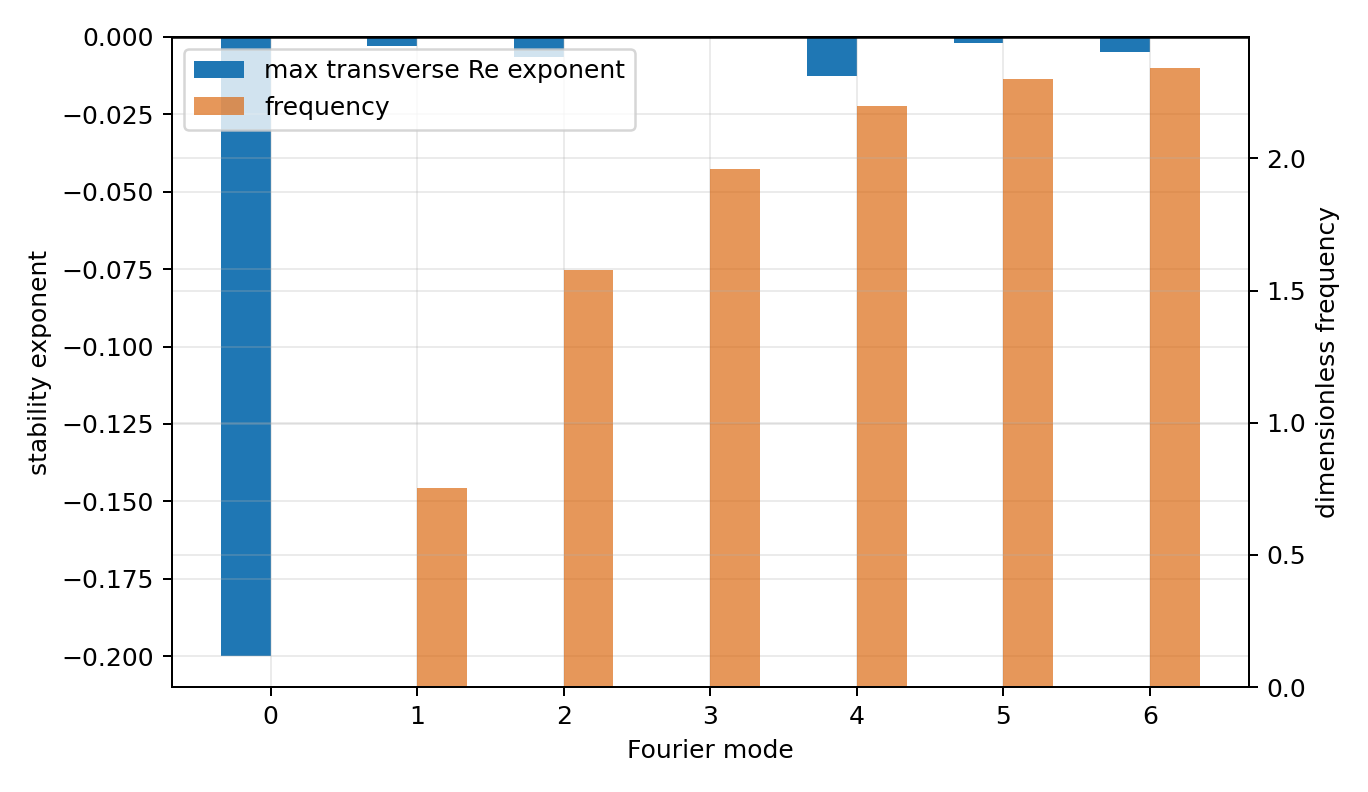
\includegraphics[width=0.86\textwidth]{FIN_Programs_488_496_Figures/p488_limit_cycle_stability.png}
\caption{Frequencies and largest transverse real exponents for the supplied saturating flow. Exact persistence and numerical stability are different claim layers.}
\end{figure}

\paragraph{Verdict.}
The batch constructs persistent self-reinforced information cycles. It does not establish a localized travelling soliton, a continuum limit, or the physical law that selects $r$ and $g$.

\section{P489 --- relational time from a persistent frequency}

Select mode $m=1$. Its recorded complex coefficient has phase
\[
z(t)=z(0)e^{-i\lambda_1t},
\qquad \lambda_1=0.75412115420708.
\]
On an interval shorter than
\[
T_1=\frac{2\pi}{\lambda_1}=8.3317982424005,
\]
an unwrapped phase defines $t$ relative to a chosen origin. Beyond one period, a single phase aliases times modulo $T_1$.

\begin{proposition}[Affine scale obstruction]
For every (c>0), the replacements
\[
A\mapsto A/c,
\qquad t\mapsto ct
\]
leave $e^{-itA}$ and every phase record unchanged. Therefore the spectral clock cannot choose an absolute time unit.
\end{proposition}

The executed check used $41$ synthetic phase samples with noise standard deviation $0.005$ radian. Linear unwrapping estimated $\lambda_1$ with relative error $3.10\times10^{-4}$. The scale-orbit residuals for $c=0.1,1,10$ were below $9.0\times10^{-16}$.

If phase error is $\epsilon_\phi$ and relative frequency error is $\epsilon_\lambda<1$, a local first-order timing bound over horizon $T$ is
\[
|\widehat t-t|
\lesssim
\frac{\epsilon_\phi/\lambda_1+T\epsilon_\lambda}{1-\epsilon_\lambda}.
\]
For $\epsilon_\phi=0.01$, $\epsilon_\lambda=10^{-3}$, and $T=0.8T_1$, this gives $0.01995$ dimensionless time units.

\paragraph{Verdict.}
The user's frequency-as-time intuition survives as a relational clock theorem. It does not create a second, select the clock mode, or prove that the physical universe uses this cycle.

\section{P490 --- adaptive learning in Stieltjes memory space}

\subsection{Context response}

Split the strict $C_{12}$ carrier into even visible and odd hidden coordinates and regularize the hidden block by $0.15I$. The normalized trace self-energy is
\[
\sigma(z)=\frac1{6}\Tr\!\left[B(zI+C)^{-1}B^T\right]
=\sum_{j=1}^{3}\frac{r_j}{z+c_j},
\]
with positive poles and residues
\[
\begin{array}{c|ccc}
j&1&2&3\\\hline
c_j&1.3210910206&1.6763637131&2.0383091819\\
r_j&0.2285756964&0.1987861899&0.0322941935.
\end{array}
\]

\begin{theorem}[Class-preserving adaptive parameterization]
Write $c_j=e^{b_j}$, $r_j=e^{a_j}$, and update $a,b$ by any finite gradient step that remains finite. Then $c_j,r_j>0$, and
\[
(-1)^k\sigma^{(k)}(z)
=k!\sum_j\frac{r_j}{(z+c_j)^{k+1}}>0
\]
for (z>0). The learned response remains in the rational Stieltjes class.
\end{theorem}

Twelve deterministic-seed random starts recovered the $48$-point trace response below $10^{-6}$; the best maximum relative error was $1.31\times10^{-15}$. Positivity margins through derivative order four remained strictly positive. The relative Jacobian condition number was $3.52\times10^7$, warning that accurate response does not imply robust pole identification.

\begin{figure}[H]
\centering
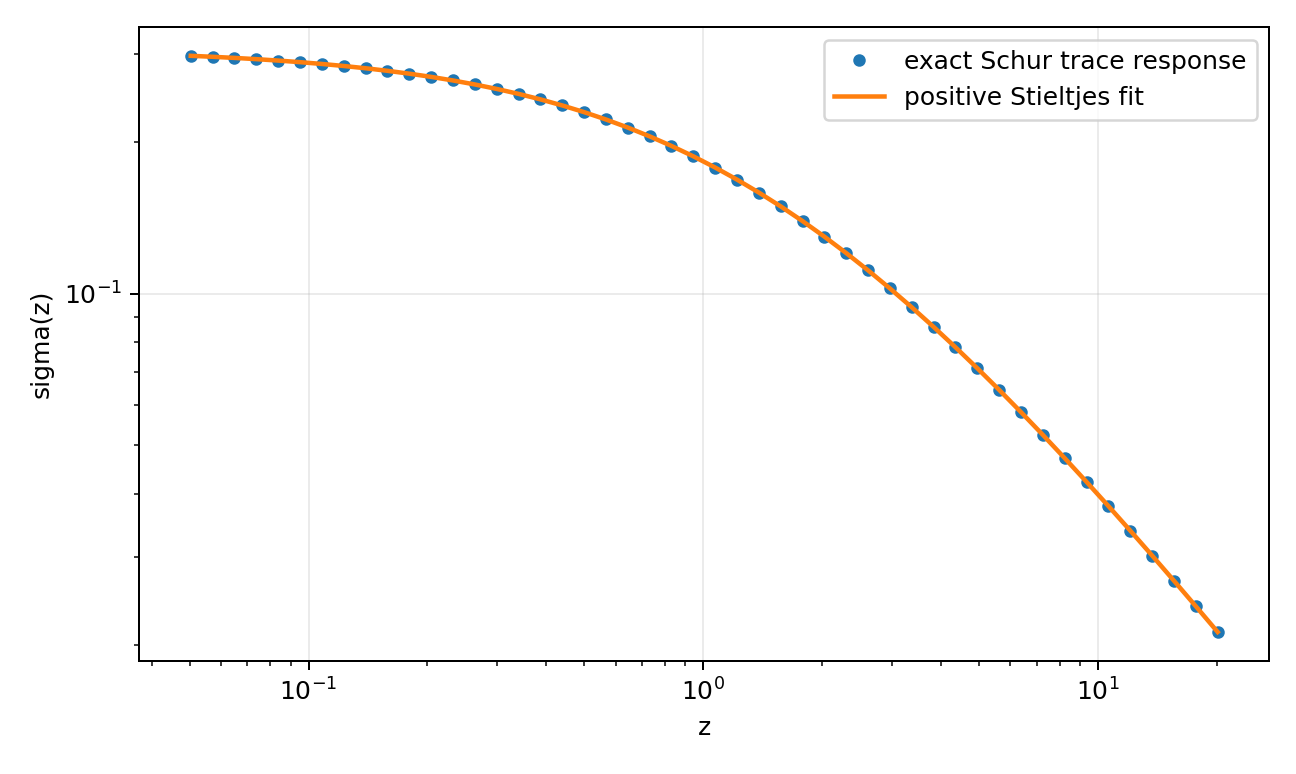
\includegraphics[width=0.82\textwidth]{FIN_Programs_488_496_Figures/p490_stieltjes_learning.png}
\caption{Exact strict Schur trace response and the learned positive three-pole Stieltjes representation.}
\end{figure}

\paragraph{Verdict.}
FIN now has a mathematically natural adaptive law in memory-function space. The construction does not internally generate its training target, loss, observations, or learning rate.

\section{P491 --- dynamic fractal fixed-point test}

To avoid importing the strict oscillatory phase outside its canonical $C_{12}$ scope, this programme declares the positive attenuation family
\[
h(d)=\frac1{1+d^{1.8}}
\]
on $C_n$, $n=12,24,48,96$. Even vertices are retained, odd vertices hidden, and $0.1I$ regularizes the hidden block. Define the scale-normalized trace fingerprint
\[
F_n(u)=\frac{\Tr[B(u\,c_nI+C)^{-1}B^T]}{\Tr[B(c_nI+C)^{-1}B^T]},
\]
where $c_n$ is the median hidden eigenvalue.

The distinct visible pole counts were
\[
3,\quad6,\quad12,\quad24,
\]
for $C_{12},C_{24},C_{48},C_{96}$. Successive maximum fingerprint differences on the seven-point $u$-grid were
\[
0.0059889,\qquad0.0129334,\qquad0.0081270.
\]

\begin{proposition}[Declared finite-family obstruction]
Two rational Stieltjes functions with positive noncancelling residues can be identical only if their pole sets and residues agree. The declared fingerprints have different visible pole counts and nonzero response differences. Hence they are not an exact dynamic fixed point of this normalization.
\end{proposition}

The discrepancies do not decrease monotonically, so these four sizes do not supply evidence of numerical convergence either. They do not prove that no different refinement, normalization or infinite-dimensional fixed point can exist.

\begin{figure}[H]
\centering
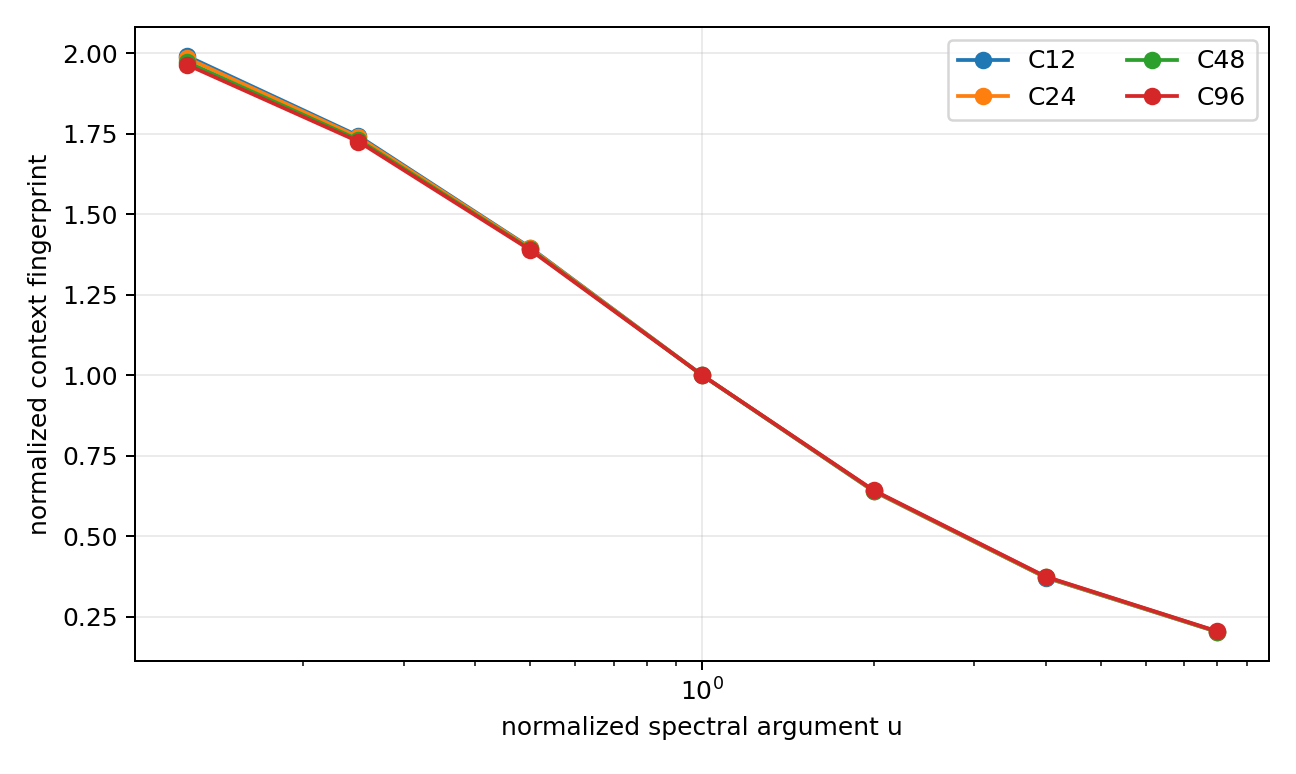
\includegraphics[width=0.82\textwidth]{FIN_Programs_488_496_Figures/p491_dynamic_context_fingerprints.png}
\caption{Normalized dynamic context fingerprints. Their proximity is approximate; pole counts exclude exact equality in the declared family.}
\end{figure}

\section{P492 --- what ``maximum resonance'' means mathematically}

\begin{theorem}[Resonance--Dirichlet complementarity]
For every nonzero $x\in\C^{12}$,
\[
\frac{\langle x,Wx\rangle}{\langle x,x\rangle}
=s-
\frac{\langle x,Ax\rangle}{\langle x,x\rangle}.
\]
Consequently maximizing coupling resonance of $W$ is exactly minimizing Dirichlet cost of $A$ on the same constraint set.
\end{theorem}

The random numerical replay residual was $8.89\times10^{-16}$; the standard-library rational checker verifies the identity exactly on 80 instances. On the mean-zero subspace,
\[
\max R_W=0.9061861245590195,
\qquad
\min R_A=0.7541211542070796,
\]
and their sum is $s$.

``Highest temporal resonance'' can instead mean maximum $A$-frequency. The paired values are
\[
\lambda_{\max}(A)=2.3421820411463004,
\qquad
\lambda_{\min}(W)=-0.6818747623802017.
\]
This criterion reverses the coupling ordering.

\begin{figure}[H]
\centering
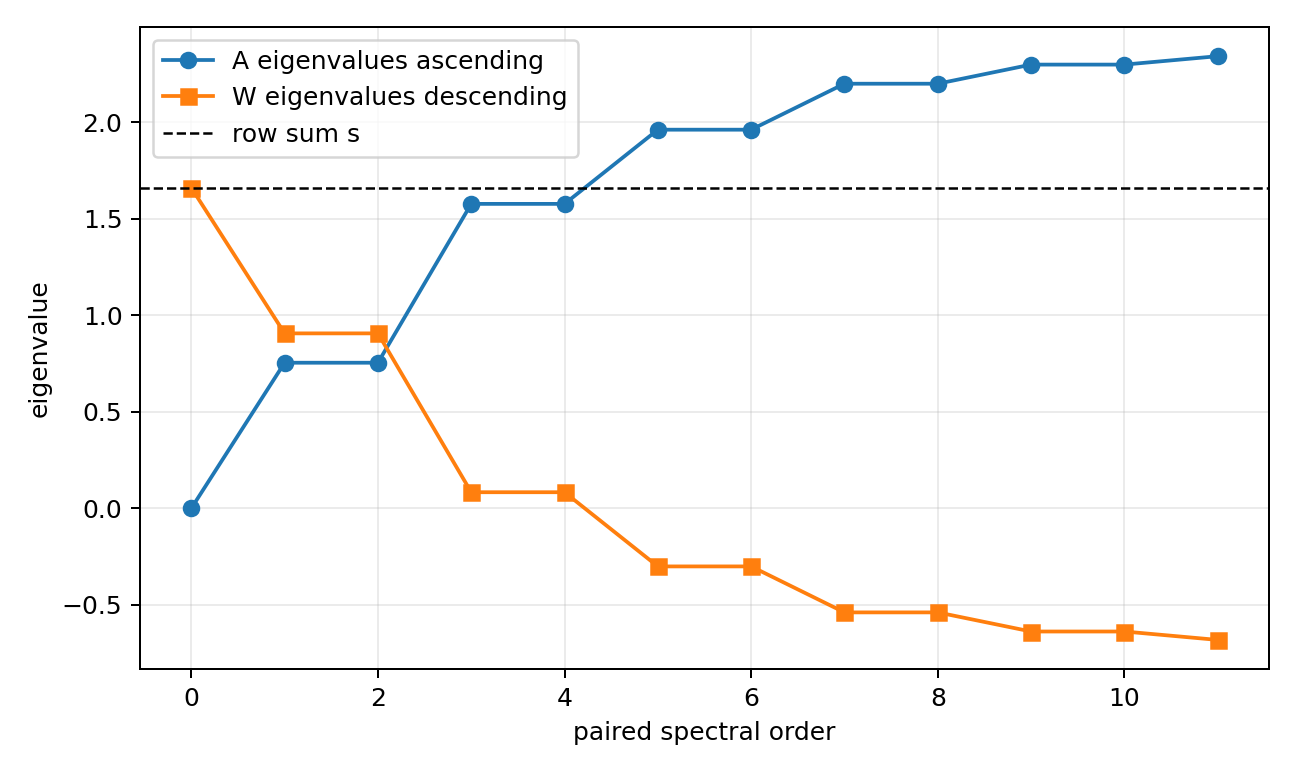
\includegraphics[width=0.82\textwidth]{FIN_Programs_488_496_Figures/p492_resonance_dirichlet.png}
\caption{Paired spectral ordering. The sum of corresponding $W$ and $A$ eigenvalues is the row sum $s$.}
\end{figure}

\paragraph{Verdict.}
The founding phrase needs a declared observable. Maximum coupling is not an alternative to minimum Dirichlet cost in the current strict model; it is the same variational statement. Sustained excitation is supplied by P488's gain--saturation law, not by spectral ordering alone.

\section{P493 --- a typed dynamic carrier for Legacy* and strict}

\subsection{Exponent-lift automaton}

For parameters $p=(a,\beta,\eta,\omega,\phi)$, define
\[
q_{d+1}=q_d+1,
\qquad
c_{d+1}=\frac{c_d}{1+\beta[(q_d+1)^\eta-q_d^\eta]c_d},
\qquad
\theta_{d+1}=\theta_d+\omega,
\]
with $q_0=0$, $c_0=1$, $\theta_0=\phi$, and output
\[
K_d=a c_d\cos\theta_d.
\]

\begin{theorem}[Exact exponent-lift representation]
For every integer $d\ge0$,
\[
c_d=\frac1{1+\beta d^\eta},
\qquad
K_d=a\frac{\cos(\omega d+\phi)}{1+\beta d^\eta}.
\]
\end{theorem}

\begin{proof}
The result is true at $d=0$. If it holds at $d$, then
\[
c_{d+1}
=\frac{1}{1+\beta d^\eta+\beta[(d+1)^\eta-d^\eta]}
=\frac1{1+\beta(d+1)^\eta}.
\]
The phase recurrence is immediate.
\end{proof}

The Legacy* point is
\[
(a,\beta,\eta,\omega,\phi)
=(4\ln2,0.01,1,\pi/4,\pi/6),
\]
while strict is
\[
(1,1,1.8,0.18575,0.16250).
\]
The automaton matched both closed forms through distance $48$ to below floating tolerance and transferred identically on $C_{12},C_{16},C_{24}$.

This is representation, not derivation: every endpoint parameter is supplied. A linear homotopy between parameter tuples retains one or more negative radial weights until the sampled parameter $t=0.93$. Therefore most of that simple path is not a nonnegative-weight passive graph Laplacian. No physical legacy role transfers through this automaton.

\paragraph{Verdict.}
The construction identifies a compact dynamic state space containing both kernel classes and isolates the missing problem as a parameter-source law. It does not solve that problem.

\section{P494 --- topology and the particle-defect boundary}

Fourier phase patterns on the cycle have discrete winding $m$ for increments strictly inside $(-\pi,\pi)$. Their strict Dirichlet energies are the spectral values:
\[
\begin{aligned}
E_{\pm1}&=0.7541212,& E_{\pm2}&=1.5770495,& E_{\pm3}&=1.9614069,\\
E_{\pm4}&=2.1995688,& E_{\pm5}&=2.2986063.&&
\end{aligned}
\]
The Nyquist mode $m=6$ lies exactly at edge increment $\pi$, so its signed winding depends on branch convention and is marked ambiguous.

\begin{theorem}[Scalar-kernel topology obstruction]
The unconstrained scalar configuration space $\C^{12}$ is contractible. Hence it has no disconnected winding sectors. A path from the $m=1$ Fourier field to the constant field can pass through the zero field with finite strict Dirichlet energy. Protected winding requires at least:
\begin{enumerate}
\item a nonvanishing $S^1$-valued phase field or equivalent target constraint;
\item a declared interpolation on cycle edges;
\item a refinement/continuum rule preserving the homotopy class.
\end{enumerate}
\end{theorem}

The finite kernel can assign energy to a supplied winding pattern; it cannot create the target space or identify that pattern with an electron, muon, tau, or any other particle.

\section{P495 --- a small operational identifiability atlas}

Four declared finite models were compared:

\begin{itemize}
\item strict unitary $\rho\mapsto e^{-itA}\rho e^{itA}$;
\item strict Markov populations $p\mapsto e^{-tA}p$;
\item vertex-dephasing Lindblad dynamics with $\gamma=0.6$;
\item a completely positive synthetic coherence-revival family
\[
\rho(t)=q(t)U_t\rho U_t^\dagger+[1-q(t)]\operatorname{diag}(U_t\rho U_t^\dagger),
\quad q(t)=0.45+0.40\cos(2.8t).
\]
\end{itemize}

Six preparations, three times and vertex/Fourier measurements were available. Multinomial records used (120) shots per context and (100) trials per true model.

\begin{center}
\begin{tabularx}{0.94\textwidth}{@{}Xrrr@{}}
\toprule
Design & Contexts & Minimum mean TV & Classification accuracy\\
\midrule
D1: one time, basis, vertex & 3 & $1.16\times10^{-18}$ & $0.5775$\\
D2: multitime, all preparations, vertex & 18 & $2.05\times10^{-17}$ & $0.7450$\\
D3: multitime, all preparations, vertex+Fourier & 36 & (0.0487983) & (1.0000)\\
\bottomrule
\end{tabularx}
\end{center}

D1 and D2 contain an exactly/near-exactly indistinguishable pair in their declared population records: dephasing a coherent state does not change its instantaneous vertex diagonal. Fourier measurement exposes the missing coherence and separates every model in this synthetic dataset.

\begin{figure}[H]
\centering
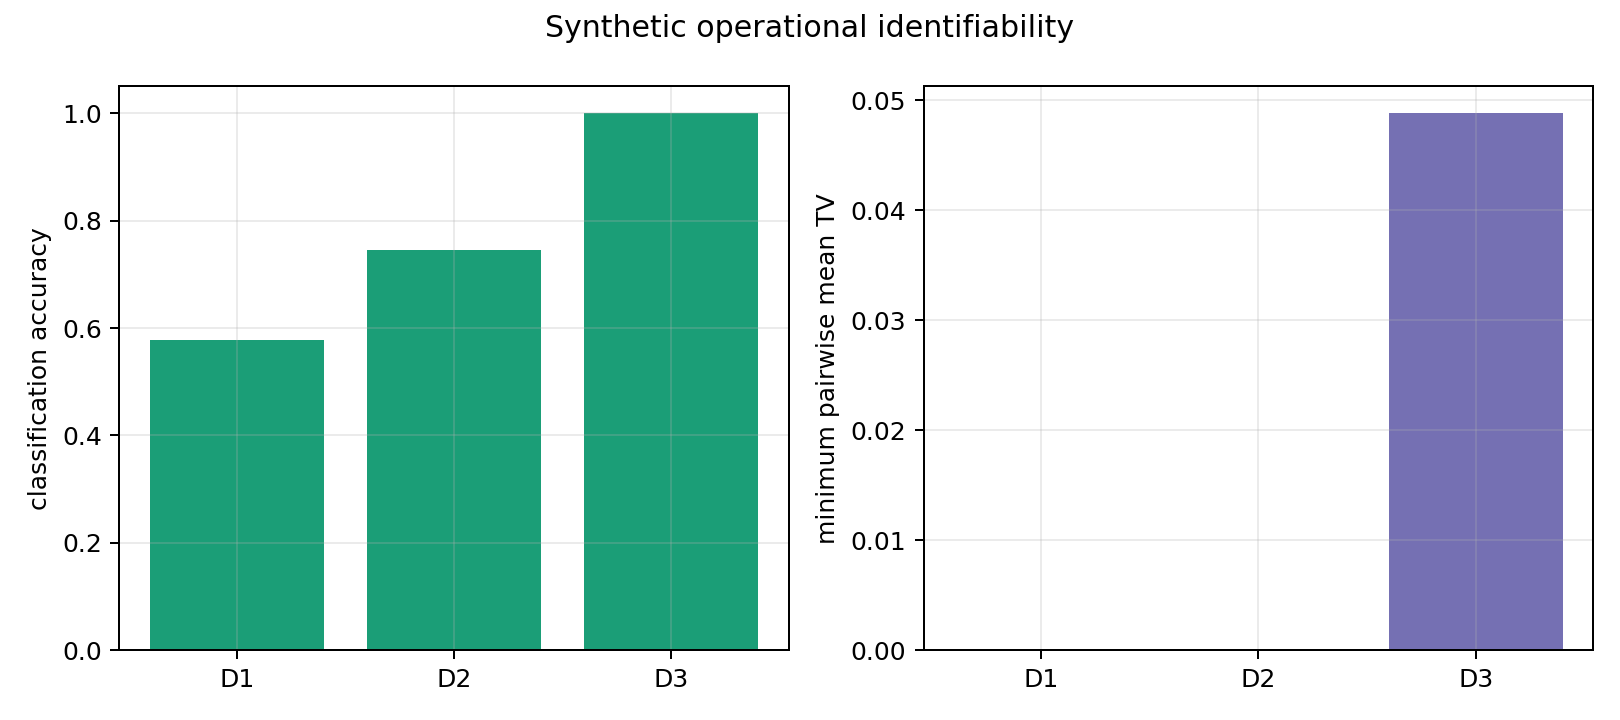
\includegraphics[width=0.78\textwidth]{FIN_Programs_488_496_Figures/p495_operational_identifiability.png}
\caption{Operational resources matter more than additional population samples for the declared unitary/revival ambiguity.}
\end{figure}

\paragraph{Verdict.}
The result supports the laboratory package's demand for informationally complete preparations and instruments. Perfect synthetic classification is not a laboratory prediction, hardware tolerance theorem, or external validation.

\section{P496 --- dependency-minimal exact replay}

The standard-library checker uses exact rational arithmetic and no NumPy, SciPy, SymPy or network resource. It passed:

\begin{itemize}
\item 80 exact regular-circulant Dirichlet identities;
\item 80 exact Rayleigh complementarity identities;
\item 60 exact positive rational Green--Schur block identities;
\item 25 exact Legacy* $\eta=1$, $\beta=1/100$ automaton steps.
\end{itemize}

The checker strengthens reproducibility and rejects accidental floating-only algebra. It is not a proof-assistant kernel, does not certify the transcendental strict decimals, and does not replace the analytic proofs stated above.

\section{Integrated consequences for FIN}

\subsection{What has genuinely improved}

\begin{enumerate}
\item \textbf{Persistence now has a concrete model.} The P488 law is the smallest executed mechanism in this batch combining positive self-reinforcement, saturation, and strict spectral phase evolution.
\item \textbf{Frequency can carry relative time.} P489 converts the user's intuition into a theorem with an explicit alias period and error ledger.
\item \textbf{Learning can occur in the right object space.} P490 adapts a Green--Schur memory response while preserving the Stieltjes cone.
\item \textbf{Legacy and strict share an exact dynamic syntax.} P493 supplies a state recurrence producing both formula classes at different parameters.
\item \textbf{The missing topology is precisely typed.} P494 identifies the nonvanishing phase field and refinement rule that particle-defect claims require.
\item \textbf{The observer needs coherence access.} P495 shows why population-only records can leave unitary and revival descriptions indistinguishable.
\end{enumerate}

\subsection{What has not improved}

\begin{itemize}
\item P488's modes are not localized solitons.
\item The gain, saturation, learning loss and clock choice are additional laws.
\item The absolute time, length and action scales remain absent.
\item No exact fractal dynamic fixed point was found in the declared family.
\item P493 does not derive strict parameters from legacy and transfers no old physical role.
\item No particle, mass, gauge field, gravity or laboratory record is generated.
\item The selector obstruction $QW\text{-}2191$ is untouched.
\end{itemize}

\claimbox{\textbf{Updated interpretation.} The most promising low-cost continuation of FIN is no longer another static kernel fit. It is a nonlinear spectral-memory theory: strict supplies the conservative phase geometry, a separately justified gain--saturation law supplies persistence, and Stieltjes--Schur state variables supply adaptive memory. Localization, parameter provenance, operational calibration, and topology remain the decisive missing theorems.}

\section{Recommended next low-compute studies P497--P506}

These recommendations remain local and bounded. They do not reopen the high-cost exact-algebra jobs.

\begin{longtable}{@{}p{0.09\textwidth}p{0.28\textwidth}p{0.45\textwidth}p{0.10\textwidth}@{}}
\caption{Next analytical/small-compute programmes.}\\
\toprule
Program & Objective & Acceptance criterion & Priority\\
\midrule
\endfirsthead
\toprule
Program & Objective & Acceptance criterion & Priority\\
\midrule
\endhead
P497 & Localized nonlinear strict states & Continue stationary solutions from a single-site anti-continuum limit; measure IPR and prove/refute persistence under strict coupling. & 10/10\\
P498 & Certified P488 stability & Enclose every nonzero real Jacobian exponent by interval arithmetic, separating the neutral $m=3$ direction. & 8/10\\
P499 & Two-frequency clock atlas & Prove periodicity versus injectivity from rational/irrational frequency ratios; quantify finite-precision recurrence. & 8/10\\
P500 & Stieltjes identifiability bounds & Convert the $3.52\times10^7$ condition number into rigorous noise-to-pole uncertainty bounds. & 9/10\\
P501 & Context-family limit test & Extend P491 to $C_{192},C_{384}$ and derive an asymptotic integral fingerprint before claiming or rejecting convergence. & 7/10\\
P502 & Exact passivity boundary & Interval-isolate the first P493 homotopy parameter with all six radial weights nonnegative and audit PSD separately. & 7/10\\
P503 & Nonvanishing phase refinement & Add an $S^1$-valued field and prove a discrete winding preservation theorem under bounded updates. & 9/10\\
P504 & Minimal coherence tester & Remove preparations/measurements from D3 until the smallest still-separating synthetic tester is certified. & 8/10\\
P505 & Formal theorem interface & Translate P488 existence, P489 scale orbit, P492 complementarity and P493 induction into a proof-assistant-neutral theorem dependency file. & 7/10\\
P506 & Parameter-source identifiability no-go & Determine which observations could identify a unique trajectory in P493 parameter space without inserting the strict endpoint. & 10/10\\
\bottomrule
\end{longtable}

P497 is scientifically the most important: localization is the missing property separating a persistent spectral oscillator from a soliton. P500 and P506 test whether the new adaptive/dynamic objects can ever become predictive rather than fitted.

\section{Reproducibility}

Primary artifacts:

\begin{itemize}
\item \path{fin_programs_488_496_low_compute.py};
\item \path{fin_programs_488_496_exact_checker.py};
\item \path{test_fin_programs_488_496.py};
\item \path{FIN_Programs_488_496_Results.json};
\item \path{FIN_Programs_488_496_Exact_Check.json};
\item \path{FIN_Programs_488_496_Summary.csv};
\item \path{FIN_Programs_488_496_Figures/}.
\end{itemize}

Local commands:

\begin{verbatim}
MPLCONFIGDIR=/tmp/fin-mpl-1048 \
  python3 fin_programs_488_496_low_compute.py
python3 -m unittest -v test_fin_programs_488_496.py
pdflatex -interaction=nonstopmode -halt-on-error \
  FIN_Programs_488_496_Low_Compute_Analytical_Report_EN.tex
\end{verbatim}

The full run used one deterministic seed, dense matrices of size at most $144\times144$, refinement matrices no larger than $96\times96$, and small nonlinear least squares. It is designed for an ordinary local computer.

\section{Final verdict and nonclaims}

The low-compute route was scientifically productive. It did not solve the most expensive exact-algebra problems, yet it constructed objects closer to the founding FIN idea than another static interpolation would have done. The strict spectrum can support persistent self-reinforced cycles after a minimal saturating law is supplied. Their frequency gives a rigorous relational clock. Hidden-state response admits a positivity-preserving learning law. Legacy* and strict fit one exact dynamic recurrence syntax. These are real mathematical advances within declared models.

The same batch sharply limits interpretation. The cycles are not localized. The clock has no absolute unit. The adaptive response is ill-conditioned and trained on supplied data. The dynamic kernel automaton imports all endpoint parameters. Scalar states have no protected particle winding. Population measurements alone do not determine the temporal model.

No result here discharges $QW\text{-}2191$, sources orientation, produces dimensional standards, completes the legacy-to-strict bridge, transfers a legacy physical role, supplies independent custody or laboratory evidence, derives particles, masses, the Standard Model, gravity, $L_{\rm total}$, or a Theory of Everything.

\end{document}
